%-----------------------------------------------------------------------------------------------------------------------------------------------%
%	The MIT License (MIT)
%
%	Copyright (c) 2019 Jan Küster
%
%	Permission is hereby granted, free of charge, to any person obtaining a copy
%	of this software and associated documentation files (the "Software"), to deal
%	in the Software without restriction, including without limitation the rights
%	to use, copy, modify, merge, publish, distribute, sublicense, and/or sell
%	copies of the Software, and to permit persons to whom the Software is
%	furnished to do so, subject to the following conditions:
%	
%	THE SOFTWARE IS PROVIDED "AS IS", WITHOUT WARRANTY OF ANY KIND, EXPRESS OR
%	IMPLIED, INCLUDING BUT NOT LIMITED TO THE WARRANTIES OF MERCHANTABILITY,
%	FITNESS FOR A PARTICULAR PURPOSE AND NONINFRINGEMENT. IN NO EVENT SHALL THE
%	AUTHORS OR COPYRIGHT HOLDERS BE LIABLE FOR ANY CLAIM, DAMAGES OR OTHER
%	LIABILITY, WHETHER IN AN ACTION OF CONTRACT, TORT OR OTHERWISE, ARISING FROM,
%	OUT OF OR IN CONNECTION WITH THE SOFTWARE OR THE USE OR OTHER DEALINGS IN
%	THE SOFTWARE.
%	
%
%-----------------------------------------------------------------------------------------------------------------------------------------------%


%============================================================================%
%
%	DOCUMENT DEFINITION
%
%============================================================================%

%we use article class because we want to fully customize the page and don't use a cv template
\documentclass[10pt,A4]{article}	


%----------------------------------------------------------------------------------------
%	ENCODING
%----------------------------------------------------------------------------------------

% we use utf8 since we want to build from any machine
\usepackage[utf8]{inputenc}		

%----------------------------------------------------------------------------------------
%	LOGIC
%----------------------------------------------------------------------------------------

% provides \isempty test
\usepackage{xstring, xifthen}

%----------------------------------------------------------------------------------------
%	FONT BASICS
%----------------------------------------------------------------------------------------

% some tex-live fonts - choose your own

%\usepackage[defaultsans]{droidsans}
%\usepackage[default]{comfortaa}
%\usepackage{cmbright}
\usepackage[default]{raleway}
%\usepackage{fetamont}
%\usepackage[default]{gillius}
%\usepackage[light,math]{iwona}
%\usepackage[thin]{roboto} 

% set font default
\renewcommand*\familydefault{\sfdefault} 	
\usepackage[T1]{fontenc}

% more font size definitions
\usepackage{moresize}

%----------------------------------------------------------------------------------------
%	FONT AWESOME ICONS
%---------------------------------------------------------------------------------------- 

% include the fontawesome icon set
\usepackage{fontawesome}

% use to vertically center content
% credits to: http://tex.stackexchange.com/questions/7219/how-to-vertically-center-two-images-next-to-each-other
\newcommand{\vcenteredinclude}[1]{\begingroup
\setbox0=\hbox{\includegraphics{#1}}%
\parbox{\wd0}{\box0}\endgroup}

% use to vertically center content
% credits to: http://tex.stackexchange.com/questions/7219/how-to-vertically-center-two-images-next-to-each-other
\newcommand*{\vcenteredhbox}[1]{\begingroup
\setbox0=\hbox{#1}\parbox{\wd0}{\box0}\endgroup}

% icon shortcut
\newcommand{\icon}[3] { 							
	\makebox(#2, #2){\textcolor{maincol}{\csname fa#1\endcsname}}
}	

% icon with text shortcut
\newcommand{\icontext}[4]{ 						
	\vcenteredhbox{\icon{#1}{#2}{#3}}  \hspace{2pt}  \parbox{0.9\mpwidth}{\textcolor{#4}{#3}}
}

% icon with website url
\newcommand{\iconhref}[5]{ 						
    \vcenteredhbox{\icon{#1}{#2}{#5}}  \hspace{2pt} \href{#4}{\textcolor{#5}{#3}}
}

% icon with email link
\newcommand{\iconemail}[5]{ 						
    \vcenteredhbox{\icon{#1}{#2}{#5}}  \hspace{2pt} \href{mailto:#4}{\textcolor{#5}{#3}}
}

%----------------------------------------------------------------------------------------
%	PAGE LAYOUT  DEFINITIONS
%----------------------------------------------------------------------------------------

% page outer frames (debug-only)
% \usepackage{showframe}		

% we use paracol to display breakable two columns
\usepackage{paracol}

% define page styles using geometry
\usepackage[a4paper]{geometry}

% remove all possible margins
\geometry{top=1cm, bottom=1cm, left=1cm, right=1cm}

\usepackage{fancyhdr}
\pagestyle{empty}

% space between header and content
% \setlength{\headheight}{0pt}

% indentation is zero
\setlength{\parindent}{0mm}

%----------------------------------------------------------------------------------------
%	TABLE /ARRAY DEFINITIONS
%---------------------------------------------------------------------------------------- 

% extended aligning of tabular cells
\usepackage{array}

% custom column right-align with fixed width
% use like p{size} but via x{size}
\newcolumntype{x}[1]{%
>{\raggedleft\hspace{0pt}}p{#1}}%


%----------------------------------------------------------------------------------------
%	GRAPHICS DEFINITIONS
%---------------------------------------------------------------------------------------- 

%for header image
\usepackage{graphicx}

% use this for floating figures
% \usepackage{wrapfig}
% \usepackage{float}
% \floatstyle{boxed} 
% \restylefloat{figure}

%for drawing graphics		
\usepackage{tikz}				
\usetikzlibrary{shapes, backgrounds,mindmap, trees}

%----------------------------------------------------------------------------------------
%	Color DEFINITIONS
%---------------------------------------------------------------------------------------- 
\usepackage{transparent}
\usepackage{color}

% primary color
\definecolor{maincol}{RGB}{ 225, 0, 0 }

% accent color, secondary
% \definecolor{accentcol}{RGB}{ 250, 150, 10 }

% dark color
\definecolor{darkcol}{RGB}{ 70, 70, 70 }

% light color
\definecolor{lightcol}{RGB}{245,245,245}


% Package for links, must be the last package used
\usepackage[hidelinks]{hyperref}

% returns minipage width minus two times \fboxsep
% to keep padding included in width calculations
% can also be used for other boxes / environments
\newcommand{\mpwidth}{\linewidth-\fboxsep-\fboxsep}
	


%============================================================================%
%
%	CV COMMANDS
%
%============================================================================%

%----------------------------------------------------------------------------------------
%	 CV LIST
%----------------------------------------------------------------------------------------

% renders a standard latex list but abstracts away the environment definition (begin/end)
\newcommand{\cvlist}[1] {
	\begin{itemize}{#1}\end{itemize}
}

%----------------------------------------------------------------------------------------
%	 CV TEXT
%----------------------------------------------------------------------------------------

% base class to wrap any text based stuff here. Renders like a paragraph.
% Allows complex commands to be passed, too.
% param 1: *any
\newcommand{\cvtext}[1] {
	\begin{tabular*}{1\mpwidth}{p{0.98\mpwidth}}
		\parbox{1\mpwidth}{#1}
	\end{tabular*}
}

%----------------------------------------------------------------------------------------
%	CV SECTION
%----------------------------------------------------------------------------------------

% Renders a a CV section headline with a nice underline in main color.
% param 1: section title
\newcommand{\cvsection}[1] {
	\vspace{14pt}
	\cvtext{
		\textbf{\LARGE{\textcolor{darkcol}{\uppercase{#1}}}}\\[-4pt]
		\textcolor{maincol}{ \rule{0.1\textwidth}{2pt} } \\
	}
}

%----------------------------------------------------------------------------------------
%	META SKILL
%----------------------------------------------------------------------------------------

% Renders a progress-bar to indicate a certain skill in percent.
% param 1: name of the skill / tech / etc.
% param 2: level (for example in years)
% param 3: percent, values range from 0 to 1
\newcommand{\cvskill}[3] {
	\begin{tabular*}{1\mpwidth}{p{0.65\mpwidth}  r}
 		\textcolor{black}{\textbf{#1}} & \textcolor{maincol}{#2}\\
	\end{tabular*}%
	
	\hspace{4pt}
	\begin{tikzpicture}[scale=1,rounded corners=2pt,very thin]
		\fill [lightcol] (0,0) rectangle (1\mpwidth, 0.15);
		\fill [maincol] (0,0) rectangle (#3\mpwidth, 0.15);
  	\end{tikzpicture}%
}


%----------------------------------------------------------------------------------------
%	 CV EVENT
%----------------------------------------------------------------------------------------

% Renders a table and a paragraph (cvtext) wrapped in a parbox (to ensure minimum content
% is glued together when a pagebreak appears).
% Additional Information can be passed in text or list form (or other environments).
% the work you did
% param 1: time-frame i.e. Sep 14 - Jan 15 etc.
% param 2:	 event name (job position etc.)
% param 3: Customer, Employer, Industry
% param 4: Short description
% param 5: work done (optional)
% param 6: technologies include (optional)
% param 7: achievements (optional)
\newcommand{\cvevent}[7] {
	
	% we wrap this part in a parbox, so title and description are not separated on a pagebreak
	% if you need more control on page breaks, remove the parbox
	\parbox{\mpwidth}{
		\begin{tabular*}{1\mpwidth}{p{0.72\mpwidth}  r}
	 		\textcolor{black}{\textbf{#2}} & \colorbox{maincol}{\makebox[0.25\mpwidth]{\textcolor{white}{#1}}} \\
			\textcolor{maincol}{\textbf{#3}} & \\
		\end{tabular*}\\[8pt]
	
		\ifthenelse{\isempty{#4}}{}{
			\cvtext{#4}\\
		}
	}

	\ifthenelse{\isempty{#5}}{}{
		\vspace{9pt}
		{#5}
	}

	\ifthenelse{\isempty{#6}}{}{
		\vspace{9pt}
		\cvtext{\textbf{Technologies include:}}\\
		{#6}
	}

	\ifthenelse{\isempty{#7}}{}{
		\vspace{9pt}
		\cvtext{\textbf{Achievements include:}}\\
		{#7}
	}
	\vspace{14pt}
}

%----------------------------------------------------------------------------------------
%	 CV META EVENT
%----------------------------------------------------------------------------------------

% Renders a CV event on the sidebar
% param 1: title
% param 2: subtitle (optional)
% param 3: customer, employer, etc,. (optional)
% param 4: info text (optional)
\newcommand{\cvmetaevent}[4] {
	\textcolor{maincol} {\cvtext{\textbf{\begin{flushleft}#1\end{flushleft}}}}

	\ifthenelse{\isempty{#2}}{}{
	\textcolor{darkcol} {\cvtext{\textbf{#2}} }
	}

	\ifthenelse{\isempty{#3}}{}{
		\cvtext{{ \textcolor{darkcol} {#3} }}\\
	}

	\cvtext{#4}\\[14pt]
}

%---------------------------------------------------------------------------------------
%	QR CODE
%----------------------------------------------------------------------------------------

% Renders a qrcode image (centered, relative to the parentwidth)
% param 1: percent width, from 0 to 1
%\newcommand{\cvqrcode}[1] {
%	\begin{center}
%		
\includegraphics[width={#1}\mpwidth]{PortfolioENPP}
%	\end{center}
%}


%============================================================================%
%
%
%
%	DOCUMENT CONTENT
%
%
%
%============================================================================%
\begin{document}
\columnratio{0.31}
\setlength{\columnsep}{2.2em}
\setlength{\columnseprule}{4pt}
\colseprulecolor{lightcol}
\begin{paracol}{2}
\begin{leftcolumn}
%---------------------------------------------------------------------------------------
%	META IMAGE
%----------------------------------------------------------------------------------------
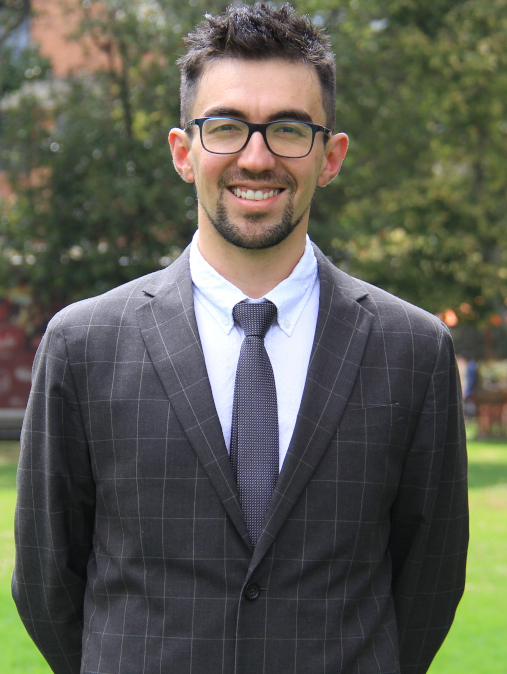
\includegraphics[width=\linewidth]{profile_photo_reduced.jpg}	%trimming relative to image size

%---------------------------------------------------------------------------------------
%	META SKILLS
%----------------------------------------------------------------------------------------
\cvsection{HARD SKILLS}

\cvskill{Python} {7+ yrs} {1} \\[-2pt]

\cvskill{Linux} {5+ yrs} {1} \\[-2pt]

\cvskill{Open Source Tools} {5+ yrs} {1} \\[-2pt]

\cvskill{Git} {4+ yrs} {0.7} \\[-2pt]

\cvskill{ROS} {3+ yrs} {0.5} \\[-2pt]

\cvskill{C++} {1+ yrs} {0.2} \\[-2pt]



\vfill\null
\cvsection{CONTACT}
	
\icontext{MapMarker}{12}{Calle 12 3 05\\251201 La Calera, Colombia}{black}\\[6pt]
\icontext{Github}{12}{nikorose87}{black}\\[6pt]
\icontext{MobilePhone}{12}{+57 300 3501177}{black}\\[6pt]
\icontext{Twitter}{12}{nikorose}{black}\\[6pt]
\iconemail{Envelope}{12}{enprietop@unal.edu.co}{enprietop@unal.edu.co}{black}\\[6pt]

\vfill\null
%\cvqrcode{0.7}

%---------------------------------------------------------------------------------------
%	EDUCATION
%----------------------------------------------------------------------------------------
\newpage

\cvsection{Personality traits}

\cvskill{Reserved}{Energetic} {0.8} \\[-2pt]

\cvskill{Cautious} {Curious} {0.8} \\[-2pt]

\cvskill{Spontaneous} {Organized} {0.85} \\[-2pt]

\cvskill{Competitive} {Friendly} {0.75} \\[-2pt]

\cvskill{Avid} {Modest} {0.9} \\[-2pt]

\cvskill{Confident} {Nervous} {0.65} \\[-2pt]


\cvsection{EDUCATION}

\cvmetaevent
{2014 - 2021}
{Ph.D in Mechatronics Engineering.}
{Universidad Nacional de Colombia}
{A complete characterization of the ankle Dynamic Joint Stiffness through the data analysis of human gait datasets available in the literature was performed at different instances.
A predictor with ML algorithms of the ankle DJS based on the anthropomorphic human features was proposed.
A dynamic computational framework for obtaining the best ankle-foot passive prosthesis was developed with FEM tools and optimized through Bayesian techniques.}

\cvmetaevent
{2011 - 2014}
{M.Sc. in Mechatronics Engineering}
{Universidad Militar Nueva Granada}
{I developed an ankle-foot prosthesis for Colombian runners with optimal combination of carbon-fiber laminates.}

\cvmetaevent
{2004 - 2009}
{B.E. in Mechatronics.}
{Universidad de San Buenaventura}
{}

%---------------------------------------------------------------------------------------
%	CERTIFICATION
%----------------------------------------------------------------------------------------
%\newpage
\cvsection{Certificates}

\cvmetaevent
{Algorithms and data structures Specialization}
{Coursera}
{1/4 courses}
{Algorithmic techniques for solving various computational problems}

\cvmetaevent
{Reinforcement Learning Specialization}
{Coursera}
{1/4 courses}
{Skills to implement a complete RL solution and understand how to apply AI tools to solve real-world problems.}

\cvmetaevent
{Deep learning Specialization}
{Coursera}
{1/4 courses}
{A foundational program that will help you understand the capabilities, challenges, and consequences of deep learning.}


\vfill
%\cvqrcode{0.7}


\end{leftcolumn}
\begin{rightcolumn}
%---------------------------------------------------------------------------------------
%	TITLE  HEADER
%----------------------------------------------------------------------------------------
\fcolorbox{white}{darkcol}{\begin{minipage}[c][3.5cm][c]{1\mpwidth}
	\begin {center}
		\HUGE{ \textbf{ \textcolor{white}{ \uppercase{ Nikolay Prieto} } } } \\[-24pt]
		\textcolor{white}{ \rule{0.1\textwidth}{1.25pt} } \\[4pt]
		\large{ \textcolor{white} {Software Developer, ML Engineer} }
	\end {center}
\end{minipage}} \\[14pt]
\vspace{-12pt}

%---------------------------------------------------------------------------------------
%	PROFILE
%----------------------------------------------------------------------------------------
\vfill\null
\cvsection{PROFILE}

\cvtext{
Ph.D. with strong knowledge in software development, computer science, design optimization, robotics, and data science. I have got work experience as a back-end engineer, project manager, researcher, and as a professor. I have excellent skills in object-oriented programming, machine learning, data science, Industrial Internet of Things (IIoT), computational robotics, computer vision, maths, embedded systems, statistics, project management, and physical computer modeling. Nowadays, I am looking for a job in the tech industry and/or research.

%good skills in personal relationships, leadership, responding flexibly and positively to changing situations, continuous learning autonomy, persistent and oriented to objectives
}

%---------------------------------------------------------------------------------------
%	WORK EXPERIENCE
%----------------------------------------------------------------------------------------
\vfill\null
\cvsection{WORK EXPERIENCE}

\cvevent
	{Nov 2021 - NOW}
	{Mvnifest}
	{Backend Engineer}
	{Mvnifest is a third-party logistics company re-inventing the way logistics is being managed. We are creating a mainframe to help with the entire process. I am a Python remote developer in this company.}
	{\cvlist{
		\item To develop Distributed Systems on the cloud for a third party logistics company.}}
	{\cvlist {
		\item Python for custom tool development.
		\item Neo4J (NoSQL) as main database framework.
		\item AWS services included: Appsync, S3, EC2, lambda, SES, SQS, SNS, SAM, API gateway, eventbridge.
	}}
	{\cvlist{
		\item In charge of the design and re-factoring of code modules from monolithic services into distributed systems.
		\item Authorization and Authentication system.
		\item Development of microservices either with REST or graphQL interfaces.
		\item Documentation and infrastructure design on templates.
	}}

\vfill\null

\cvevent
	{Jul 2019 - Dec 2021}
	{Universidad de San Buenaventura}
	{Computational Robotics and AI}
	{Associate professor of undergraduate and graduate program in the mechatronics department. My research is focused on the development of machines (robots) with Computer Vision and/or Machine Learning integration algorithms.}
	{\cvlist{
		\item Non Linear control of the ankle dynamic joint stiffness predicted via XGBoost algorithm.
		\item Development of an autonomous mobile robot for food services.
		\item Development of a 3D printer with IoT integration.
		\item Visual Inertial Navigation systems for aereal and ground autonomous vehicles. 
	}}
	{\cvlist {
		\item Python for custom tool development.
		\item Pandas, Scikit-learn, OpenCV, ROS, Gazebo, jupyter, Google Colab, keras, tensorflow, CAD.
	}}
	{\cvlist{
		\item Two (2) Industrial Prototypes.
		\item One (1) Back-end application.
	}}

\vfill\null
\cvevent
	{Aug 14 - Aug 19}
	{Universidad Nacional de Colombia}
	{Engineering Design researcher}
	{Doctoral researcher focused on the analysis of the ankle dynamics and design of ankle-foot prostheses using advanced design methods as surrogate models and transient simulations of solid materials.}
	{\cvlist{
		\item An ankle dynamic joint stiffness profile predictor from anthropomorphic measurements with ensemble algorithms.
		\item An optimal ankle-foot prosthesis shape generator according to their age, race and gait speed using Bayesian optimization. 
	}}
	{\cvlist {
		\item Python for custom tool development.
		\item ANSYS, LS-DYNA, Linux environment.
		\item Use of IU servers to enhance the process performance. 
		\item QD, pandas, scikit-learn, scikit-posthoc, scikit-fda, VTK, scipy, researchpy, google colab, tensorflow, keras.
		\item Git for configuration and documentation versioning.
	}}
	{\cvlist{
		\item Best GPA 2015-I during doctoral studies.
		\item Full scholarship from MINCIENCIAS for PhD studies.
		\item Two (2) back-end open source applications to be used by the research community. 
	}}

%\vfill\null
\cvevent
	{Jun 18 - Dec 18}
	{Indiana University Purdue University Indianapolis.}
	{Research Assistant}
	{I performed activities including the following:}
	{\cvlist{
		\item Design and construction of a catheter holder for medical applications through additive manufacturing and injection plastic processes.
		\item Physically testing of the medical devices at different configurations.
		\item Attend lectures in relevant topics such as topology optimization.
	}}
	{\cvlist {
		\item Linux and Python for custom Tool development.
		\item LS-DYNA, BayesOpt, scikit-optimize.
	}}
	{\cvlist{
		\item One (1) final report of medical design.
		\item One (1) Industrial prototype to begin test on users.
	}}

%\vfill\null
\cvevent
	{Feb 09 - Sep 14}
	{Military Industry of Colombia.}
	{Research and Development Project Manager}
	{Administrative and technical management of projects focused on researchand technological development in the defense field. The duties involved were:}
	{\cvlist{
		\item Management of five (5) research projects. Total investment of two (2) million dollars.
		\item Monitoring transfer of the generated know-how to the implied factories.
		\item Technological assessment,industrial property, engineering design and manufacturing of prototypes.
	}}
	{\cvlist {
		\item Microsoft Project, Office 365.
		\item Inventor, solidworks.
		\item Altium Designer, Matlab. 
	}}
	{\cvlist{
		\item Two (2) TV operated mobile robot prototypes.
		\item A variety of prosthetics for lower and upper limbs.
		\item Development of command and control systems for the Colombian navy.
		\item One (1) military vehicle prototype.
		\item Master Scholarship by the Military Industry.
	}}


% hotfixes to create fake-space to ensure the whole height is used
\mbox{}
\vfill
\mbox{}
\vfill
\mbox{}
\vfill
\mbox{}
\end{rightcolumn}
\end{paracol}
\end{document}

